\documentclass{beamer}

\usepackage[french]{babel}
\usepackage[T1]{fontenc}
\usepackage[utf8]{inputenc}

\usetheme{Warsaw}
\useoutertheme{infolines}

\usepackage{amsmath}
\usepackage{amssymb}
\usepackage{amsthm}
\usepackage{stmaryrd}

\usepackage{listings}
\usepackage{color}

\definecolor{mygreen}{rgb}{0,0.6,0}
\definecolor{mygray}{rgb}{0.5,0.5,0.5}
\definecolor{mymauve}{rgb}{0.58,0,0.82}

\lstset{ %
  backgroundcolor=\color{white},   % choose the background color
  basicstyle=\footnotesize,        % size of fonts used for the code
  breaklines=true,                 % automatic line breaking only at whitespace
  captionpos=b,                    % sets the caption-position to bottom
  commentstyle=\color{mygreen},    % comment style
  escapeinside={\%*}{*)},          % if you want to add LaTeX within your code
  keywordstyle=\color{blue},       % keyword style
  stringstyle=\color{mymauve},     % string literal style
}

\lstset{language=java} 

\usepackage[all]{xy}

%Les sous listes on des triangles
\setbeamertemplate{itemize item}[circle]
\setbeamertemplate{itemize subitem}[triangle]
%Les elements caché sont grisé
\beamertemplatetransparentcovered

\begin{document}

\title{Android - Tâches asynchrones}
\author{Jérémy S. Cochoy}
\institute{INRIA Paris-Saclay | jeremy.cochoy@gmail.com}
\date{Decembre 2015}


\begin{frame}
\titlepage
\end{frame}

\begin{frame}
\frametitle{Sommaire}
\tableofcontents
\end{frame}

\begin{frame}
\frametitle{La documentation}
\begin{center}

\includegraphics[scale=0.5]{livres.png}
\end{center}
\begin{block}{Votre nouveau livre de chevet.}
\begin{center}
\emph{https://developer.android.com/guide/index.html}
\end{center}
\end{block}

\end{frame}

\section{La classe AsyncTask}

\begin{frame}
\frametitle{\verb!AsyncTask!}
\begin{center}
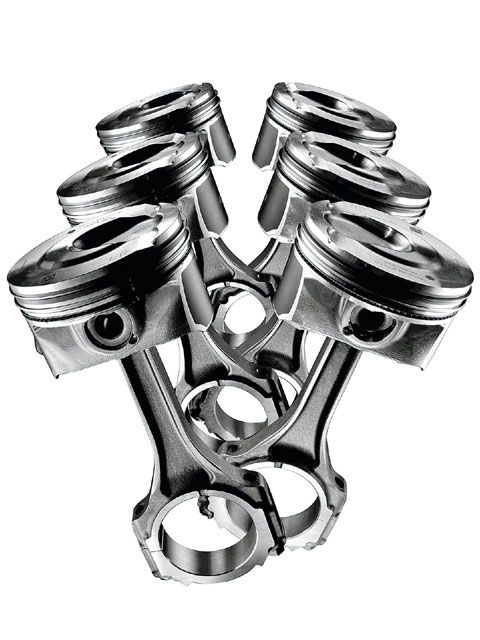
\includegraphics[scale=0.07]{async.jpg}
\end{center}
\begin{block}{Pour effectuer une tâche asynchrone...}
Pour exécuter une tâche de quelques secondes, on utilise la classe \verb!AsyncTask! qui contiendra le code à exécuter en parallèle de l'activité en cours.
\end{block}
\pause
\begin{block}{}
C'est une classe générique!
\end{block}
\pause
\begin{exampleblock}{On hérite de \verb!AsyncTask!}
 private class DownloadFilesTask extends AsyncTask<URL, Integer, Long> { ... }
\end{exampleblock}
\end{frame}

\begin{frame}
\frametitle{Types génériques}

\begin{center}

\includegraphics[scale=0.5]{generic.jpg}
\end{center}
\begin{block}{Les types utilisés par \verb!AsyncTask! sont :}

\begin{itemize}
\item Params - Le type des arguments passés au thread lors de son lancement.
\item Progress - Le type de l'unité de mesure de la progression communiqué durant le calcul en arrière-plan.
\item Result - Le type du résultat renvoyé après le calcul.
\end{itemize}

\end{block}
\end{frame}

\subsection{Le corps}
\begin{frame}
\frametitle{\verb!doInBackground()!}
\begin{block}{Où placer la tâche couteuse ?}
La tâche à effectuer en arrière-plan se place dans \verb!doInBackground!.
\end{block}
\pause
\begin{block}{Arguments et retour}
Elle prend un(des) argument(s) de type \emph{Params} et renvoie un résultat de type \emph{Result}.
\end{block}
\pause
\begin{block}{VarArgs}
Le nombre d'arguments est variable. On les récupère sous la forme d'un tableau.
\end{block}
\end{frame}

\begin{frame}
\frametitle{\verb!doInBackground()!}
\begin{block}{\verb!La méthode isCancelled()!}
Lors de l'exécution de votre tâche, c'est à vous de réagir dans le cas où celle-ci est annulée dans l'activité principale via la méthode \verb!cancel()!. Pour cela, regardez la valeur de retour de \verb!isCancelled()!.
\end{block}
\pause
\begin{block}{La méthode \verb!publishProgress!}
A chaque modification du niveau de progression de votre tâche, c'est à vous de communiquer cette information via \verb!publishProgress()!.
\end{block}
\end{frame}

\begin{frame}[fragile]
\begin{exampleblock}{Exemple de \verb!doInBackground!}
\begin{lstlisting}
protected Long doInBackground(URL... urls)
{
  int count = urls.length;
  long totalSize = 0;
  for (int i = 0; i < count; i++) {
    totalSize += Downloader.downloadFile(urls[i]);
    publishProgress((int) ((i / (float) count) * 100));
    // Fin de l'execution si cancel()est appelee.
    if (isCancelled()) break;
  }
  return totalSize;
}
\end{lstlisting}
\end{exampleblock}
\end{frame}

\subsection{Communication}
\begin{frame}[fragile]
\frametitle{\verb!onProgressUpdate()!}
\begin{block}{La méthode \verb!onProgressUpdate()!}
C'est la méthode appelée lors d'une évolution de la progression. Elle s'exécute dans le thread de l'activité et peut donc accéder à ses variables membres.
\end{block}
\begin{exampleblock}{Exemple de \verb!onProgressUpdate()!.}
\begin{lstlisting}
protected void onProgressUpdate(Integer... progress)
{
  mProgressBar.setProgress(progress[0]);
}
\end{lstlisting}
\end{exampleblock}
\end{frame}

\subsection{Pre / Post exécution}
\begin{frame}[fragile]
\frametitle{Pre-process}

\begin{block}{\verb!onPreExecute()!}
\verb!onPreExecute! est exécutée avant le traitement de la tâche. Elle est appelée dans le thread de l'activité.
\end{block}

\begin{exampleblock}{Exemple :}
\begin{lstlisting}
protected void onPreExecute()
{
  //Traitement a effectuer
}
\end{lstlisting}
\end{exampleblock}
\end{frame}
\begin{frame}[fragile]
\frametitle{Post-process}

\begin{block}{\verb!onPostExecute()!}
\verb!onPostExecute! est exécutée après le traitement de la tâche. Elle est appelée dans le thread de l'activité.
\end{block}

\begin{exampleblock}{Exemple :}
\begin{lstlisting}
protected void onPostExecute(Long result)
{
  showDialog("Downloaded " + result + " bytes");
}
\end{lstlisting}
\end{exampleblock}
\end{frame}

\begin{frame}[fragile]
\frametitle{Exécuter notre tâche}

\begin{block}{\verb!execute()!}
Pour exécuter notre tâche, on crée une instance de notre classe et on appelle la méthode \verb!execute()!.
\end{block}
\begin{exampleblock}{Exemple :}
\begin{lstlisting}
private class DownloadFilesTask extends
              AsyncTask<URL, Integer, Long> { ... }

// Pour executer notre tache asynchrone :
new DownloadFilesTask().execute(url1, url2, url3);
\end{lstlisting}
\end{exampleblock}

\end{frame}

\section{Alternatives}
\subsection{Thread et Handler}

\begin{frame}
\begin{center}

\includegraphics[scale=0.2]{thread.jpg}
\end{center}
\frametitle{Thread et Handler}

\begin{block}{Thread}
La classe \verb!Thread! permet l'exécution asynchrone d'une tâche pouvant se maintenir durant tout le temps de vie de l'application.
On peut dériver \verb!Thread! et surcharger \verb!run()!, ou bien passer un objet de type \verb!Runnable!.
\end{block}

\begin{block}{Handler}
La classe \verb!Handler! permet la communication entre les threads (notamment entre le thread de l'activité et un de vos threads), via un système de queue de messages.
\end{block}

\end{frame}

\subsection{Executor}
\begin{frame}
\begin{center}

\includegraphics[scale=0.25]{executor.jpg}
\end{center}
\begin{block}{Executor}
Pour gérer l'exécution de plusieurs tâches sans devoir explicitement créer les threads, jetez un œil à \verb!Executor!.
\end{block}
\begin{block}{ThreadPoolExecutor}
Si vous avez un nombre important de tâches à exécuter, jetez un œil à \verb!ThreadPoolExecutor!.
\end{block}

\end{frame}


\section{Conclusion}

\begin{frame}
\frametitle{Conclusion}
\begin{block}{Les tâches asynchrones}
Les tâches asynchrones vous permettent d'effectuer des opérations couteuses comme le téléchargement de fichiers, des requêtes à une base de données, des calculs couteux en performance, etc. sans provoquer le blocage de votre activité.
\end{block}
\end{frame}

\begin{frame}
\begin{center}
Pour me contacter : jeremy.cochoy@gmail.com, merci et à bientôt.

\medskip
\medskip
\medskip
\medskip


\includegraphics[scale=0.3]{android.jpg}
\end{center}
\end{frame}




\end{document}